\chapter{Introduction}
\label{chap:introduction}

\section{Motivation}

Modern networked applications are increasingly organized as collections of
services rather than as single monolithic programs. A mobile robot may expose
telemetry, perception, and flight-control services. A ground station may provide
object detection, mapping, mission planning, and storage services. Edge devices
may request AI inference services from nearby accelerators or cloud nodes. In
each case, the application developer wants to invoke named services and retrieve
named results without manually binding every operation to a fixed host address,
a long-lived channel, and a single provider.

Today's service frameworks provide valuable engineering tools, but TCP/IP
communication is still centered on reaching endpoints and maintaining channels.
Remote procedure call (RPC) systems, REST services, and microservice platforms
typically identify service endpoints by host addresses, ports, or channel
endpoints. Robotics middleware provides publish-subscribe or request-response
communication, but often assumes an operational domain where identity, trust,
network reachability, and service discovery are configured outside the service
invocation itself. The problem is not that these tools are unusable; the problem
is that mobile and data-heavy applications want to name the service and the data
objects involved in the workflow, while the networking substrate mainly exposes
where an endpoint is and how to keep a path to it. When applications become
mobile, intermittent, multi-provider, and security-sensitive, developers must
rebuild mechanisms for discovery, retry, authorization, integrity verification,
data retrieval, and provider selection.

Named Data Networking (NDN) offers a different foundation. NDN names data
directly, secures Data packets directly, and decouples retrieval from fixed
endpoints. These properties naturally match service-oriented applications in
which users care about a named service, a named model artifact, a named
telemetry object, or a named video segment rather than a particular IP
connection. However, NDN by itself is a networking architecture, not a complete
service framework. Application developers still need a runtime that defines how
to publish service requests, authorize users and providers, select one or more
providers, protect service data, and support higher-level collaboration.

This gap also emerged from the application-driven development in this
dissertation. Building the UAV application exposed the need for stable service
selection, command authorization, telemetry freshness, local service
composition, and large video/recording object handling. Building the
distributed inference workload exposed the need to coordinate artifact
provisioning, tensor dependencies, provider roles, and large intermediate data.
These experiences motivate treating the gap as a framework problem rather than
as isolated application glue code.

\section{NDN Building Blocks for NDNSF}

This proposal assumes several NDN concepts, but they are used here for a
specific purpose: to explain why NDNSF is a data-centric service framework. NDN
is receiver-driven: a consumer sends an Interest packet for a named object, and
the network returns a matching Data packet from a producer, cache, or other
available source~\cite{ndn}. This basic exchange is not yet a complete service
invocation, but it supplies the communication primitive that NDNSF builds on:
the application names what it wants, not the host that should send it; the
returned Data packet is independently named and signed; and retrieval can
succeed even when the original producer is not on the same path as the consumer.

NDN names have three roles that are important for this dissertation. First,
they identify application data, such as telemetry, video segments, model
artifacts, service requests, ACKs, selections, and responses. Second, they are
part of the security model: trust schemas and access-control attributes can be
defined over name prefixes. Third, they guide routing and forwarding because
Interests are forwarded by name prefix rather than by destination address.
NDNSF uses the same naming foundation for service-level objects, so a service
workflow can refer to both actions and large data by name.

NDN forwarders maintain three data structures that are important for NDNSF's
design. The Forwarding Information Base (FIB) forwards Interests by name
prefix. The Pending Interest Table (PIT) records unsatisfied Interests and
aggregates multiple Interests for the same name, allowing one returned Data
packet to satisfy multiple consumers. The Content Store (CS) caches Data
packets for future retrieval. Together, these structures support stateful
forwarding, in-network caching, multicast-style delivery, and adaptive
retrieval under mobility or failures~\cite{yi2013case}. For service
applications, this means that service-related data can be named and retrieved
independently of a fixed address or connection. Service invocation semantics,
however, still have to be built above these packet and forwarding primitives.

NDN is data-centric in its security model as well as in its naming and
forwarding model. Each Data packet carries a producer signature, allowing
consumers to verify integrity and producer authenticity regardless of whether
the Data came from the original producer, an in-network cache, or a
repository~\cite{ndn}. This property is central to NDNSF: service requests,
ACKs, selections, responses, permissions, and large artifacts can all be treated
as named and verifiable objects. However, signatures alone do not decide who is
allowed to call a service, which provider is authorized to offer it, or which
attributes should protect each service message. Those higher-level decisions
are framework responsibilities.

\begin{figure}[H]
\centering
\resizebox{\textwidth}{!}{%
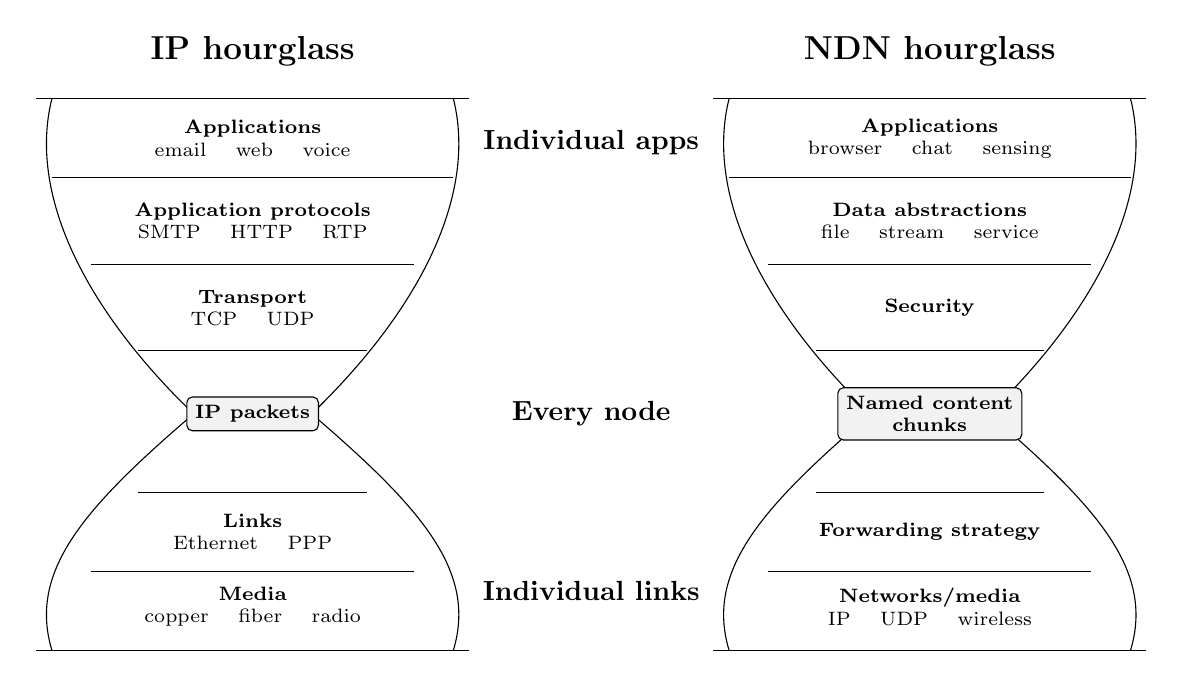
\begin{tikzpicture}[font=\scriptsize, every node/.style={align=center}]
\tikzset{
  layertext/.style={font=\scriptsize, align=center},
  waist/.style={fill=gray!10, draw, rounded corners=2pt, inner sep=3pt}
}
\begin{scope}[shift={(0,0)}]
  \node[font=\bfseries\large] at (0,5.25) {IP hourglass};
  \draw[rounded corners=2pt] (-2.75,4.65) -- (2.75,4.65);
  \draw[rounded corners=2pt] (-2.75,-2.35) -- (2.75,-2.35);
  \draw (-2.55,4.65)
    .. controls (-2.85,3.45) and (-2.15,2.00) .. (-0.75,0.65)
    .. controls (-2.15,-0.55) and (-2.85,-1.35) .. (-2.55,-2.35);
  \draw (2.55,4.65)
    .. controls (2.85,3.45) and (2.15,2.00) .. (0.75,0.65)
    .. controls (2.15,-0.55) and (2.85,-1.35) .. (2.55,-2.35);
  \foreach \y/\w in {3.65/5.10,2.55/4.10,1.45/2.90,-0.35/2.90,-1.35/4.10}
    \draw (-\w/2,\y) -- (\w/2,\y);
  \node[layertext] at (0,4.15) {\textbf{Applications}\\email \quad web \quad voice};
  \node[layertext] at (0,3.10) {\textbf{Application protocols}\\SMTP \quad HTTP \quad RTP};
  \node[layertext] at (0,2.00) {\textbf{Transport}\\TCP \quad UDP};
  \node[waist] at (0,0.65) {\textbf{IP packets}};
  \node[layertext] at (0,-0.85) {\textbf{Links}\\Ethernet \quad PPP};
  \node[layertext] at (0,-1.80) {\textbf{Media}\\copper \quad fiber \quad radio};
\end{scope}

\begin{scope}[shift={(8.6,0)}]
  \node[font=\bfseries\large] at (0,5.25) {NDN hourglass};
  \draw[rounded corners=2pt] (-2.75,4.65) -- (2.75,4.65);
  \draw[rounded corners=2pt] (-2.75,-2.35) -- (2.75,-2.35);
  \draw (-2.55,4.65)
    .. controls (-2.85,3.45) and (-2.15,2.00) .. (-0.75,0.65)
    .. controls (-2.15,-0.55) and (-2.85,-1.35) .. (-2.55,-2.35);
  \draw (2.55,4.65)
    .. controls (2.85,3.45) and (2.15,2.00) .. (0.75,0.65)
    .. controls (2.15,-0.55) and (2.85,-1.35) .. (2.55,-2.35);
  \foreach \y/\w in {3.65/5.10,2.55/4.10,1.45/2.90,-0.35/2.90,-1.35/4.10}
    \draw (-\w/2,\y) -- (\w/2,\y);
  \node[layertext] at (0,4.15) {\textbf{Applications}\\browser \quad chat \quad sensing};
  \node[layertext] at (0,3.10) {\textbf{Data abstractions}\\file \quad stream \quad service};
  \node[layertext] at (0,2.00) {\textbf{Security}};
  \node[waist] at (0,0.65) {\textbf{Named content}\\\textbf{chunks}};
  \node[layertext] at (0,-0.85) {\textbf{Forwarding strategy}};
  \node[layertext] at (0,-1.80) {\textbf{Networks/media}\\IP \quad UDP \quad wireless};
\end{scope}

\node[font=\bfseries, fill=white, inner sep=2pt] at (4.3,4.10) {Individual apps};
\node[font=\bfseries, fill=white, inner sep=2pt] at (4.3,0.65) {Every node};
\node[font=\bfseries, fill=white, inner sep=2pt] at (4.3,-1.60) {Individual links};
\end{tikzpicture}%
}
\caption{Conceptual comparison of IP and NDN hourglass models, redrawn from the NDN architecture discussion~\cite{ndn}.}
\label{fig:ndn-hourglass}
\end{figure}

\begin{figure}[H]
\centering
\resizebox{0.92\textwidth}{!}{%
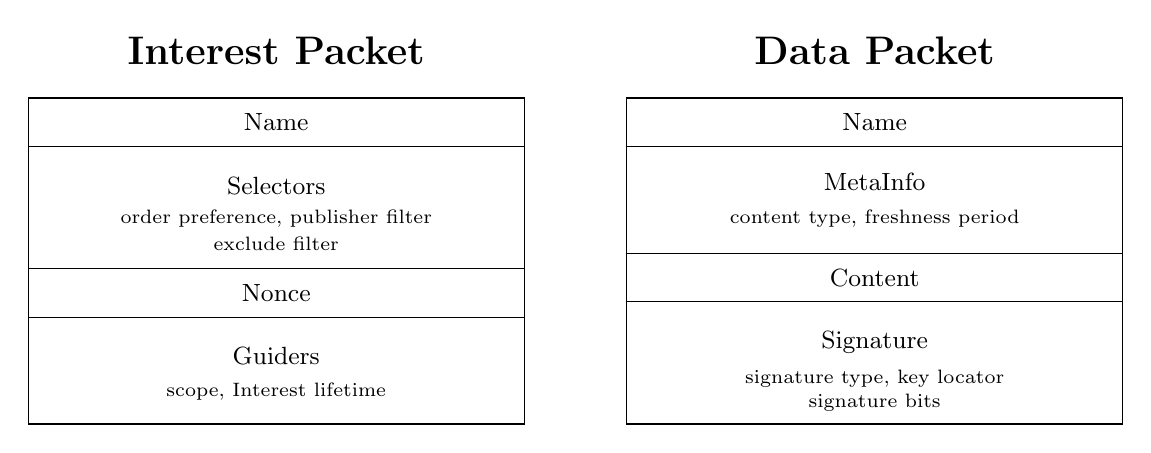
\begin{tikzpicture}[font=\small, every node/.style={align=center}]
\def\w{6.3}
\def\xA{-6.6}
\def\xB{1.0}
\node[font=\Large\bfseries] at (-3.45,2.95) {Interest Packet};
\draw (\xA,2.35) rectangle ++(\w,-0.62);
\node at (-3.45,2.04) {Name};
\draw (\xA,1.73) rectangle ++(\w,-1.55);
\node at (-3.45,1.24) {Selectors};
\node[font=\scriptsize] at (-3.45,0.82) {order preference, publisher filter};
\node[font=\scriptsize] at (-3.45,0.50) {exclude filter};
\draw (\xA,0.18) rectangle ++(\w,-0.62);
\node at (-3.45,-0.13) {Nonce};
\draw (\xA,-0.44) rectangle ++(\w,-1.35);
\node at (-3.45,-0.92) {Guiders};
\node[font=\scriptsize] at (-3.45,-1.38) {scope, Interest lifetime};

\node[font=\Large\bfseries] at (4.15,2.95) {Data Packet};
\draw (\xB,2.35) rectangle ++(\w,-0.62);
\node at (4.15,2.04) {Name};
\draw (\xB,1.73) rectangle ++(\w,-1.35);
\node at (4.15,1.28) {MetaInfo};
\node[font=\scriptsize] at (4.15,0.82) {content type, freshness period};
\draw (\xB,0.38) rectangle ++(\w,-0.62);
\node at (4.15,0.07) {Content};
\draw (\xB,-0.24) rectangle ++(\w,-1.55);
\node at (4.15,-0.76) {Signature};
\node[font=\scriptsize] at (4.15,-1.22) {signature type, key locator};
\node[font=\scriptsize] at (4.15,-1.52) {signature bits};
\end{tikzpicture}%
}
\caption{Simplified NDN Interest and Data packet structure, redrawn from the NDN architecture paper~\cite{ndn}.}
\label{fig:ndn-packets}
\end{figure}

Receiver-driven retrieval and in-network caching are useful, but service
invocation needs more than fetching a single object. Multiple providers may
need to learn that a request has been published, users may need to collect ACK
metadata before selecting providers, and long-running work may need status
diagnosis. NDNSF therefore uses NDN Sync, especially State Vector Sync as
implemented by NDN-SVS, to let users and providers discover newly published
service messages without binding the service to one fixed endpoint
~\cite{li2018brief,moll2022sok,ndnsvs-github}. In NDNSF, Sync is not the
service semantics itself; it is the dissemination substrate over which the
framework publishes Request, ACK, Selection, and Response messages as named
Data.

The implementation is built on the standard NDN software stack. NFD provides
the local forwarder and face abstraction, while \texttt{ndn-cxx} provides the
C++ application library for names, packets, faces, signing, validation, and
segmented object retrieval~\cite{ndn-cxx}. These libraries allow NDNSF to use
ordinary NDN names and packets rather than inventing a separate transport
format. They also make it possible for applications to pass large artifacts by
reference: models, video recordings, images, logs, and intermediate inference
data can be segmented into named Data packets, signed, optionally encrypted,
retrieved by name, and verified outside the small service-request payload.

For access control, NDNSF builds on NAC-ABE, which combines NDN naming with
attribute-based encryption so that service-level authorization can be expressed
over names rather than transport connections~\cite{dulal2023nacabe}. NDNSF uses this
capability together with controller-issued permissions, service-level
attributes, and per-invocation tokens. The result is that NDN supplies the
data-centric communication substrate, while NDNSF supplies the service-layer
runtime: who may call a service, who may provide it, how providers are
selected, how messages are protected, and how large named objects are attached
to service workflows.

\begin{table}[H]
\centering
\caption{How NDN building blocks motivate NDNSF mechanisms.}
\label{tab:ndn-to-ndnsf}
\begin{tabularx}{\textwidth}{p{0.28\textwidth}X}
\toprule
NDN Building Block & NDNSF Mechanism \\
\midrule
Data packets & Request, ACK, Selection, and Response are service message
objects carried as named Data. \\
Interests & Interests fetch named Data; NDN-SVS uses Sync Interests to
announce dataset updates. \\
Data signatures and name-based trust & Service messages, permissions, and
large objects can be verified independently of the path or cache that returned
them. \\
FIB/PIT/CS forwarding and caching & Service-related data can be retrieved by
name and remain meaningful across mobility, caching, and intermittent
connectivity. \\
NDN Sync / SVS & Users and providers discover newly published service events
without binding a service to a fixed endpoint. \\
Segmented Data retrieval & Large models, videos, logs, and intermediate
tensors are carried by reference rather than embedded in small service
payloads. \\
NAC-ABE and named attributes & Service-level permissions and confidentiality
policies are expressed over names and attributes rather than transport
channels. \\
\bottomrule
\end{tabularx}
\end{table}

\section{Research Gap}

The research gap is therefore between NDN communication primitives and
service-oriented application semantics. NDN provides the right lower-level
building blocks: named Data, signatures, caching, forwarding state, segmented
retrieval, and Sync-based discovery. A service framework must organize these
building blocks into a consistent higher-level runtime.

This proposal structures the gap into four layers. At the \emph{invocation
layer}, a user needs to publish a service request, collect ACK metadata, and
select one or more providers. At the \emph{authorization layer}, users and
providers need service-level permissions, name-based attributes, replay
protection, and verifiable responses. At the \emph{coordination layer}, multiple
providers may need to advertise readiness, cooperate on one task, or compose
local and remote services. At the \emph{data layer}, services need to attach
large objects such as video, model files, logs, and intermediate tensors by
name rather than carrying them inside small request payloads.

NDNSF addresses this layered gap by treating service invocation, authorization,
provider selection, collaboration, and large-data reference handling as reusable
framework mechanisms rather than application-specific glue code.

\section{Thesis Statement}

This dissertation argues that dynamic service-oriented applications expose a
recurring mismatch between TCP/IP's connection-oriented model and
service-oriented applications' data-centric needs: applications want to operate
on named services, named data, and verifiable results, while the network stack
usually exposes addresses, channels, and endpoints. A data-centric service
framework can close this gap by making service invocation, authorization,
provider selection, collaboration, and large-object retrieval explicit
framework-level abstractions over NDN names and verifiable Data packets.

NDNSF v0.1 is a completed core contribution of this dissertation and
demonstrates the feasibility of this direction. The remaining dissertation work
extends this foundation into a framework for real dynamic service applications
and evaluates it through two high-pressure domains with different service
requirements:

\begin{itemize}
  \item \textbf{UAV network applications} represent mobile, command-sensitive,
  real-time service-container workloads, where intermittent connectivity,
  command authorization, telemetry, live video, recording, object detection,
  and multi-UAV missions must be coordinated across a ground station and
  multiple drones.
  \item \textbf{Distributed AI inference} represents artifact-heavy,
  multi-stage compute/data collaboration workloads, where model shards, runtime
  artifacts, intermediate tensors, large-data objects, and heterogeneous inference
  providers must be selected, verified, and coordinated.
\end{itemize}

\section{Research Questions}

The dissertation is organized around the following research questions.

\begin{enumerate}[label=RQ\arabic*., leftmargin=*]
  \item What problems in host-centric service frameworks can be addressed by
  data-centric service frameworks?
  \item How should NDNSF expose service invocation, authorization, provider
  selection, collaboration, and large-object retrieval as generic framework
  abstractions without forcing each application to design a custom NDN
  protocol?
  \item What reliability, security, and latency tradeoffs arise when NDN
  service requests are published to multiple providers and resolved through ACK
  metadata, provider selection, and collaboration, and how should supporting
  mechanisms such as Targeted invocation and compensation be used?
  \item How can UAV network applications evaluate NDNSF under mobile,
  command-sensitive, real-time service-container workloads?
  \item How can distributed AI inference evaluate NDNSF under artifact-heavy,
  multi-stage compute/data collaboration workloads?
\end{enumerate}

\subsection{Expected Answer Shape}

The dissertation is expected to answer these questions in the following form.
RQ1 should identify a set of recurring service-application problems that are
not merely implementation gaps in existing systems, but consequences of
binding services to hosts, sessions, or channels. RQ2 should show that NDNSF
can expose service invocation, authorization, provider selection, and provider
collaboration as reusable framework mechanisms, with local composition and
large-data references serving as supporting abstractions rather than
application-specific NDN protocols. RQ3 should characterize when
one-to-many request publication, ACK metadata, provider selection, and provider
collaboration improve reliability, and when supporting mechanisms such as
Targeted invocation or compensation are needed to control latency and recovery
costs without weakening security checks. RQ4 should show that UAV workloads exercise the same framework
mechanisms under mobility, command sensitivity, real-time video, and
multi-drone collaboration. RQ5 should show that distributed inference exercises
the same mechanisms under artifact provisioning, tensor dependency exchange,
provider role assignment, and long-running distributed execution.

\section{Expected Contributions}

The expected dissertation contributions are:

\begin{enumerate}[leftmargin=*]
  \item A review and gap analysis of service-oriented application frameworks
  with a focus on why dynamic, secure, collaborative applications still require
  a new data-centric framework.
  \item The design and implementation of NDNSF as a generic dynamic C++ service
  framework over NDN.
  \item Extensions to NDNSF centered on provider collaboration, with
  supporting mechanisms for targeted invocation, trusted local service
  composition, and large-data references.
  \item A UAV service-container application over NDNSF, including flight
  control, telemetry, video, encrypted recording, object detection, and
  collaborative patrol services.
  \item A distributed AI inference application over NDNSF, including model
  splitting, service plans, reference-based artifact exchange, and automatic
  collaboration-plan generation.
  \item An evaluation of NDNSF and the application prototypes using MiniNDN,
  SITL-based UAV experiments, and selected real-machine validation.
\end{enumerate}

\section{Proposal Scope Boundary}

For clarity, this proposal treats NDNSF v0.1 as a completed core contribution
of the dissertation, not as the final complete system. NDNSF v0.1 establishes
the basic architecture and feasibility of a data-centric service framework. The
remaining dissertation work extends this foundation into an
application-validated framework. The main framework extension is provider
collaboration: how multiple authorized providers discover requests, advertise
capabilities, are selected, exchange state or artifacts, and jointly complete a
service task. Targeted invocation, trusted local invocation, and large-data
references are treated as supporting mechanisms that make this collaborative
service model practical under low-latency, same-process composition, and
large-object workloads. These mechanisms are not UAV-only or AI-only features;
they are proposed NDNSF framework mechanisms whose usefulness will be evaluated
through two demanding application classes.

The core dissertation question is therefore not whether two applications can
be built, but whether NDNSF can provide reusable data-centric service
mechanisms that remain valid across two very different workloads.

The UAV application is used to validate NDNSF as a service-container framework
for mobile, command-sensitive, real-time systems. Its design exercises typed
telemetry, mission, video, and safety information; Targeted flight-control
commands; adaptive live video; encrypted local recording; object-detection
service composition; and multi-drone patrol workflows. The DistributedInference
application is used to validate NDNSF as a framework for artifact-heavy,
multi-stage compute/data collaboration. Its design exercises automatic model
plan generation, reference-based model and activation artifacts, predictable
prefetchable object names, and dependency-driven execution over tensor DAGs.
The dissertation therefore does not present UAV and DistributedInference as
isolated demos; it uses them as two complementary stress tests for the same
data-centric service framework thesis.

These applications also contribute requirements back to NDNSF. The UAV
workload stresses low-latency command invocation, structured command status,
service-container composition, and large-data video references, while the
DistributedInference workload stresses dependency-driven collaboration,
artifact references, provider role assignment, and long-running selection
diagnosis. Thus the application work has two roles in the dissertation: it is
valuable in its own domains, and it is the primary method for validating and
refining provider collaboration as the central NDNSF extension.
